\documentclass{anstrans}
%%%%%%%%%%%%%%%%%%%%%%%%%%%%%%%%%%%
\title{Recovering Topology of Nested Volumes Represented by Single Closed Surfaces}
\author{Chelsea A. D'Angelo, Andrew Davis, Paul P. H. Wilson}

\institute{
Computational Nuclear Engineering Research Group, University of Wisconsin-Madison, Madison WI}

\email{cadangelo@wisc.edu, andrew.davis@wisc.edu, paul.wilson@wisc.edu}

%%%% packages and definitions (optional)
\usepackage{graphicx} % allows inclusion of graphics
\usepackage{booktabs} % nice rules (thick lines) for tables
\usepackage{microtype} % improves typography for PDF

\newcommand{\SN}{S$_N$}
\renewcommand{\vec}[1]{\bm{#1}} %vector is bold italic
\newcommand{\vd}{\bm{\cdot}} % slightly bold vector dot
\newcommand{\grad}{\vec{\nabla}} % gradient
\newcommand{\ud}{\mathop{}\!\mathrm{d}} % upright derivative symbol

\begin{document}
%%%%%%%%%%%%%%%%%%%%%%%%%%%%%%%%%%%%%%%%%%%%%%%%%%%%%%%%%%%%%%%%%%%%%%%%%%%%%%%%
\section{Introduction}
As scientific computing abilities continue to advance, so too have the efforts to model
and simulate highly complex geometries in radiation environments.  Modeling has
advanced from primitive constructive solid geometry (CSG) to voxelized models, and now to high fidelity polygon mesh 
models.  While polygon mesh surface models are very accurate, most Monte Carlo codes
do not allow for their direct use. Often they are converted to voxel or tetrahedral 
mesh models and then used with the physics codes \cite{tetmesh}.

The Direct Accelerated Geometry Monte Carlo (DAGMC) software package
has the ability to efficiently run transport calculations directly on tessellated
surface models \cite{dagmc}.  Typically the surface meshes used for DAGMC 
calculations come from CAD based geometry models generated by solid modeling software.
In some cases geometries of interest, like human phantoms, are generated by other 
means and may not contain all of the necessary information for particle transport. 
For example, mesh geometries in the OBJ file format contain vertex and connectivity
data for each surface, but do not have any information about surface topology.  
These types of file formats necessitate a tool that can build a hierarchy of 
surfaces and reconstruct the topological information.  The \texttt{generate\_hierarchy} 
tool was developed for this purpose.  The following summary will explain the algorithm
behind the tool, describe a test case, and finally demonstrate a real-world application
of the tool with an MCNP5 calculation that directly uses a polygon mesh human phantom.
%%%%%%%%%%%%%%%%%%%%%%%%%%%%%%%%%%%%%%%%%%%%%%%%%%%%%%%%%%%%%%%%%%%%%%%%%%%%%%%%
\section{Methods}

%Workflow
The full workflow for a radiation transport calculation directly on a surface mesh model
employs several tools that are embedded in the Mesh Oriented datABase (MOAB) software library\cite{moab}.
MOAB is used to store the unstructured mesh data 
and has many useful built in functions for organizing the mesh data into sets, 
tagging the sets with metadata, and creating relationships between sets.  The radiation transport step relies 
on topological information about the relationships between adjacent volumes separated by the surface mesh.
When the mesh is generated directly from CAD-based geometry, the necessary topological information
is automatically incorporated into the metadata.  However, when the surface mesh is generated in other
ways, that topological information is frequently absent.  The OBJ file format\cite{obj} is a common format for
representing polygon surface mesh so capability was
added to MOAB's file readers to support it.  While this format allows for volumes to be
nested topologically, it does not include any information to describe the topology.  A separate capability
was added to MOAB's tools to reconstruct the topology once loaded into a MOAB instance.
If the geometry is going to be used 
for a Monte Carlo transport calculation, the University of Wisconsin Unified Workflow (\texttt{UW2}) can be used to attach 
the material information to the geometry file.  At this point, the geometry file
can be used with any of the DAGMC physics codes: MCNP, Fluka, and Geant4.

% ReadOBJ
\subsection{OBJ File Reader}
The basic components of a mesh geometry file are vertex coordinates and connectivity data.
The specific contents of a Wavefront OBJ file \footnote{There was a challenge in identifying an official OBJ file specification.  
With this in mind, the OBJ file reader explicitly defines which conventions it is assuming in order to eliminate some ambiguity.}
can vary and the OBJ file reader was written to support a subset of the full structure. 

The supported line types include \texttt{object}, \texttt{group},
\texttt{face}, and \texttt{vertex}.  These four types are common to many OBJ
files and contain the fundamental information needed to represent a surface
mesh geometry.  \texttt{Objects} and \texttt{groups} are both collections of
\texttt{faces}.  The important convention established here is that a
\texttt{group} is a generic collection of \texttt{faces}, while
\texttt{objects} are thought to be a collection of \texttt{faces} that form a
closed surface.  OBJ files are organized such that all mesh data that follow
an \texttt{object} or \texttt{group} line belong to that \texttt{object} or
\texttt{group}.  When an \texttt{object} or \texttt{group} line is found, a
new MOAB meshset is created and all the entities that follow become members of
that meshset.  The meshsets for \texttt{groups} are assigned a name and
ID tag.  Because \texttt{objects} are defined to represent closed volumes, the
meshset that contains the \texttt{faces} represents the surface that bounds
that volume, and an additional meshset is created to represent the volume
itself.  The volume and surface meshsets are connected through a parent-child
relationship.  In addition to a name and ID, these meshsets are also given a
category and dimension tag.  Instead of adding the \texttt{vertices} to individual
meshsets, they are added to a global vertex meshset.

% Generate Hierarchy 
\subsection{Topology Reconstruction}
For successful radiation transport, all space needs to be explicitly defined
as belonging to a volume, and only one volume.  Geometry files that only
contain surface mesh data have inadequate information to define the
relationships of those surfaces with their neighboring volumes.  In
particular, they generally can be topologically related to the volumes that
they enclose, but not to the volumes that may enclose them.  Therefore, when
one volume encloses another, the space within the enclosed volume is defined
to be part of both. \texttt{Generate\_hierarchy} is a tool within MOAB
\cite{genhi} that was created to determine the hierarchical topological
relationships among volumes and then add metadata to encode those topological
relationships, thus allowing the space in the enclosed volume to be excluded
from the outer volume.  The \texttt{generate\_hierarchy} tool has two main
public-facing functions: \texttt{build\_hierarchy} to discover the topological
relationships and \texttt{construct\_topology} to record these relationships as
metadata according to the conventions for using mesh geometry for Monte
Carlo radiation transport.

The example depicted in figure~\ref{fig:spheres}, a 2D slice of nested spheres, will 
be used to explain the algorithm for building surface hierarchy. Consider surface B.
It is completely enclosed by surface A, encloses surface D, and is beside surface C. 
These hierarchical relationships are necessary so that volumetric entities can be
determined.  For example, it can now be inferred that volume B is the space enclosed 
by surface B, but outside of surface D.

\begin{figure}[ht]
 \centering
 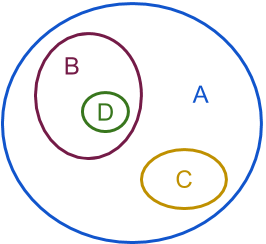
\includegraphics[width=0.22\textwidth]{../figs/nested_spheres.png}
 \caption{Two-dimensional slice of nested spheres.}
 \label{fig:spheres}
\end{figure}

In the following description of functions, surface meshsets and their corresponding volume meshsets will
together be referred to as objects.  
There are a few fundamental assumptions made by the tool about the geometry:
\begin{enumerate}
\item each surface meshset represents a single closed surface,
\item there are no overlapping/intersecting surfaces, 
\item the only topological relationships that already exist are the parent-child links between a volume meshset and its surface meshset, 
\item that topological relationship declares the volume to be 'inside' its corresponding surface mesh.
\end{enumerate}

\texttt{Build\_hierarchy} tests every object in the geometry and decides where
it belongs in a hierarchical tree.  As each new volume is added to the tree, a
breadth-first traversal is performed.  At each node in that traversal, a test
is performed to determine if the new volume encloses that node, is enclosed by
that node, or neither.  The DAGMC function \texttt{point\_in\_volume} is used
to first test whether an arbitrary vertex on the surface of one volume is
inside the other volume (and vice versa).

Whenever a new volume encloses a node, its sibling nodes are also tested to
determine whether or not they are also enclosed.  Note that once volumes are
determined to be siblings in the tree, it is not possible for them to ever
acquire a parent-child relationship, regardless of the insertion of other
volumes.  When a new volume is enclosed by a node, the tree is descended to
begin testing against another set of sibling volumes.  If a new volume neither
encloses nor is enclosed by a node, the sibling nodes are tested in the same
manner.  If there are no remaining siblings, the new volume becomes a new
sibling of those nodes in the tree.

Looking again at figure~\ref{fig:spheres}, let us assume that object A is the
first to be tested. The tree is initially empty so volume meshset A is
automatically placed at the top.  Assume object C is tested next.  The point
on its surface is found to be inside of volume A, so it becomes a child of A.
Object D is next and found to also be inside volume A, but neither inside or
outside of volume C.  Volume D becomes another child of A and sibling of C.
Last, object B is inserted. It is found to be inside of A but encloses D,
becoming a child of volume A and a parent of volume D. Because a volume can
only have one parent, the parent-child linkage between volume A and volume D
is broken.  Recall that volume D was previously considered a sibling of volume C,
so volume C must be tested for the possibility that it is also enclosed by
volume B. The test reveals that C is not in B, so the search is complete and all
volumes have been properly inserted into the tree.  
The constructed tree is shown in figure \ref{fig:tree} below.

\begin{figure}[ht] % replace 't' with 'b' to force it to be on the bottom
  \centering
  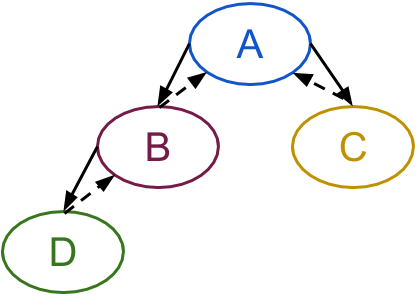
\includegraphics[width=0.25\textwidth]{../figs/tree.png}
  \caption{Hierarchical tree built from nested spheres geometry.  Arrows represent parent-child links.}
  \label{fig:tree}
\end{figure}

After the hierarchical topology has been established, DAGMC conventions are
applied to the volumes by \texttt{construct\_topology}.  This is accomplished
by setting the surface sense with respect to the enclosing volumes and
creating parent-child links between the surface meshsets and their enclosing
volumes.  Each surface has two volumes associated with it, one inside and one
outside.  As mentioned earlier, the surface sense for the 'inside' volume is
already set.  This function completes the surface sense data by setting the
'outside' volume to the enclosing volume.  Looking at figure \ref{fig:tree},
the 'inside' volume for surface B is set volume B and the 'outside' volume is
now set to volume A, the parent of volume B.  Because surface A is the
outermost surface, the 'inside' volume sense is set to volume A but the
'outside' volume sense will be empty.  Surfaces that have an empty volume
sense are interpretted during the radiation transport step to be connected to
an implicit complement.

In order to test that the correct hierarchy and topology were generated
by these tools, a test problem of six nested cubes very similar to the spheres
depicted in figure \ref{fig:spheres} was created, but with four hierarchical
levels.  Each cube was represented by a single surface and volume meshset and
all other assumptions of a pre-\texttt{generate\_hierarchy} geometry were
upheld.  In order to test the robustness of the tools, the cubes were placed
into the tree using every permutation of the ordering to confirm that the same
hierarchical relationships were established each time.

%%%%%%%%%%%%%%%%%%%%%%%%%%%%%%%%%%%%%%%%%%%%%%%%%%%%%%%%%%%%%%%%%%%%%%%%%%%%%%%%
\section{Demonstration: Surface Mesh Human Phantom}

In order to demonstrate a real-world use case, these tools were used to
prepare a polygon surface mesh human phantom for an MCNP5 calculation.  The
human phantom was developed at the Hanyang University Radiation Engineering Lab (HUREL) and provided in the OBJ file
format.  The OBJ file contained all of the vertex coordinates
and connectivity data grouped by object.  The objects in this case are parts
of the body including organs, muscle, bone, etc.  The OBJ file reader was used
to read in the file and \texttt{generate\_hierarchy} to instate the correct
hierarchical relationships and topology.  Part of the tree built by \texttt{generate\_hierarchy}
is shown in figure~\ref{fig:trimtree} below.  The full tree of 168 volumes is too large to
show here, so these particular branches were chosen in order to highlight the key features of the 
hierarchy.  The three volumes in contact with the outside
world, the skin and two corneas, are attached to the root node at the top of the tree.  
There are several layers of skin below until the residual is reached. The residual
functions as an explicit compliment that is in contact with 71 body volumes.
These 71 child volumes have varying degrees of internal structure, with some that have no children,
others that have 1-7 children, and others that contain deeply nested child volumes.  The deepest branch, 14 levels,
contains volumes in the respiratory system and is shown on the far right.

\begin{figure}[ht]
 \centering
 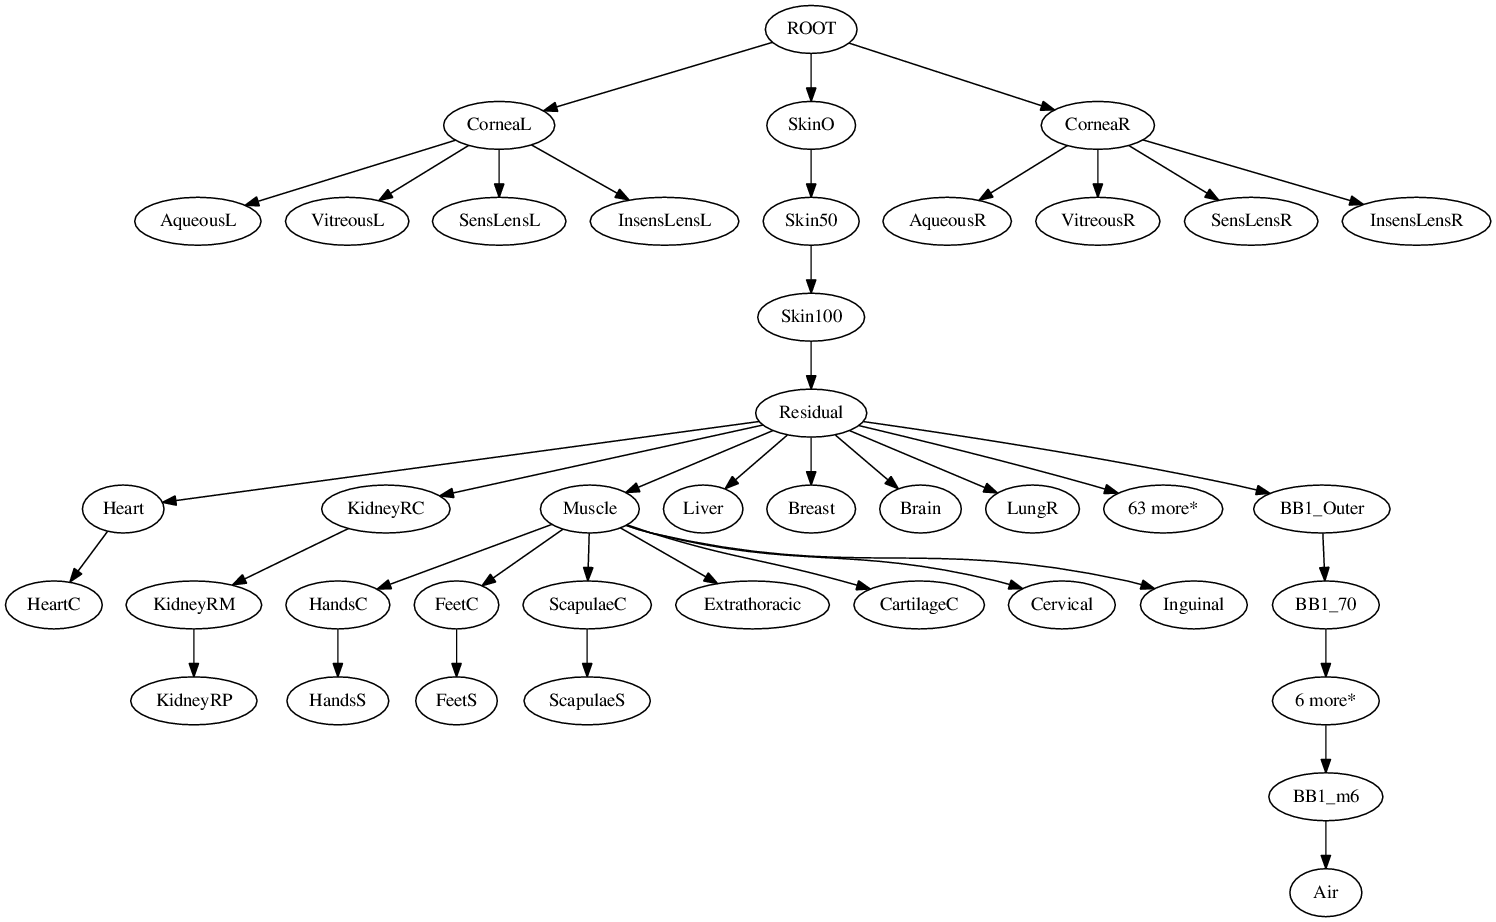
\includegraphics[width=0.5\textwidth]{../figs/trimtree.png}
 \caption{Subset of the hierarchical tree of human phantom volumes.  
          There are 63 child volumes of the residual not shown. 
          The branch of respiratory volumes on the far right also goes
          four levels deeper than what is shown here.}
 \label{fig:trimtree}
\end{figure}

The compositions for each phantom volume were provided by HUREL and the \texttt{UW2} 
process was used to attach the materials to the resulting
geometry file.

%Figure~\ref{fig:phan_mats} shows a slice of the phantom head and torso with the volumes colored
%by material.  

%\begin{figure}[ht]
% \centering
% \includegraphics[width=0.2\textwidth]{../figs/phantom_mat1.png}
% \caption{Slice of the phantom head and torso.  Each volume is colored by material.}
% \label{fig:trimtree}
%\end{figure}

For proof of concept, a DAG-MCNP calculation using a 30 KeV photon
source in the chest was performed.  The resulting mesh tally of photon flux is 
shown in figure \ref{fig:mcnp}. 

\begin{figure}[ht] % replace 't' with 'b' to force it to be on the bottom
  \centering
  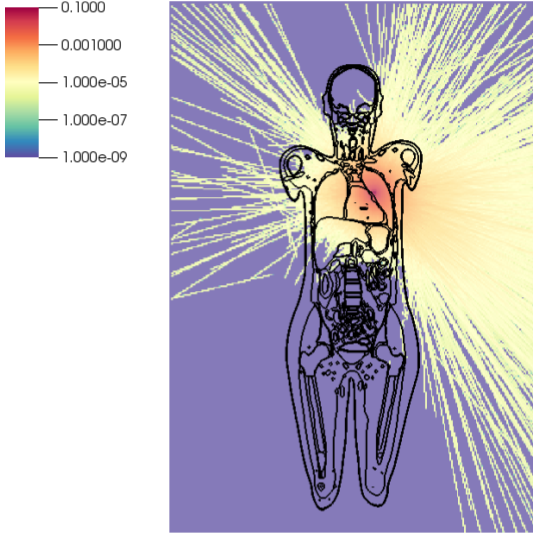
\includegraphics[width=0.4\textwidth]{../figs/30KeV_Psource.png}
  \caption{Photon flux from DAG-MCNP calculation with 30 keV photon source in chest. }
  \label{fig:mcnp}
\end{figure}


%%%%%%%%%%%%%%%%%%%%%%%%%%%%%%%%%%%%%%%%%%%%%%%%%%%%%%%%%%%%%%%%%%%%%%%%%%%%%%%%
\section{Conclusions and Future Work}

The \texttt{UW2} was developed with the goal of simulating the same Monte
Carlo problem with several physics codes so in the near future, we will run
this exact geometry in a FluDAG and DAG-Geant calculation. We will also be
able to compare the performance of the DAGMC-based polygon mesh phantom with
other representations, including voxelized and tetrahedral volume mesh, in a
number of different Monte Carlo radiation transport codes.

%%%%%%%%%%%%%%%%%%%%%%%%%%%%%%%%%%%%%%%%%%%%%%%%%%%%%%%%%%%%%%%%%%%%%%%%%%%%%%%%
\section{Acknowledgments}

The authors would like to acknowledge Dr. Chan Hyeong Kim from the Hanyang University Radiation Engineering Lab (HUREL)
for access to the mesh-type ICRP reference computational phantom currently under development by his research group.
This work was sponsored, in part by, NASA's Space Radiation Analysis Group (via Wyle Corporation grant T73043)
and the USDOE's Office of Fusion Energy Sciences (DE-FG02-99ER54513DE-FG02-99ER54513).

%%%%%%%%%%%%%%%%%%%%%%%%%%%%%%%%%%%%%%%%%%%%%%%%%%%%%%%%%%%%%%%%%%%%%%%%%%%%%%%%
\bibliographystyle{ans}
\bibliography{bibliography}
\end{document}

